\section{Design d'interfaces de l'application}

Pour montrer les nouvelles fonctions définies et vérifier la possibilité d'en réaliser, j'ai mis en oeuvre un design d'interfaces de l'application qui comprend 3 parties principales: 

\subsection{Créer un projet}

Il y a deux façon de créer un projet :

\begin{figure}[H]
\centering
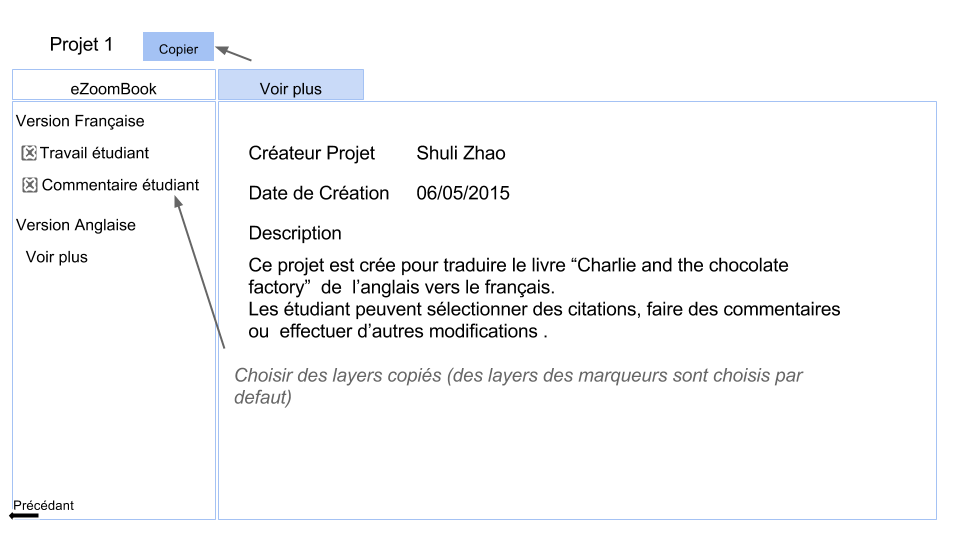
\includegraphics[width=\textwidth]{creer_projet}
\caption{Créer un projet à partir d'un projet existant}
\end{figure}

Quand on crée un projet à partir d'un projet existant, il faut choisir des layers publics à copier. Des layers originaux, des marqueurs et des séquences sont aussi conpiés automatiquement sans des informations d'éditeurs. 

\begin{figure}[H]
\centering
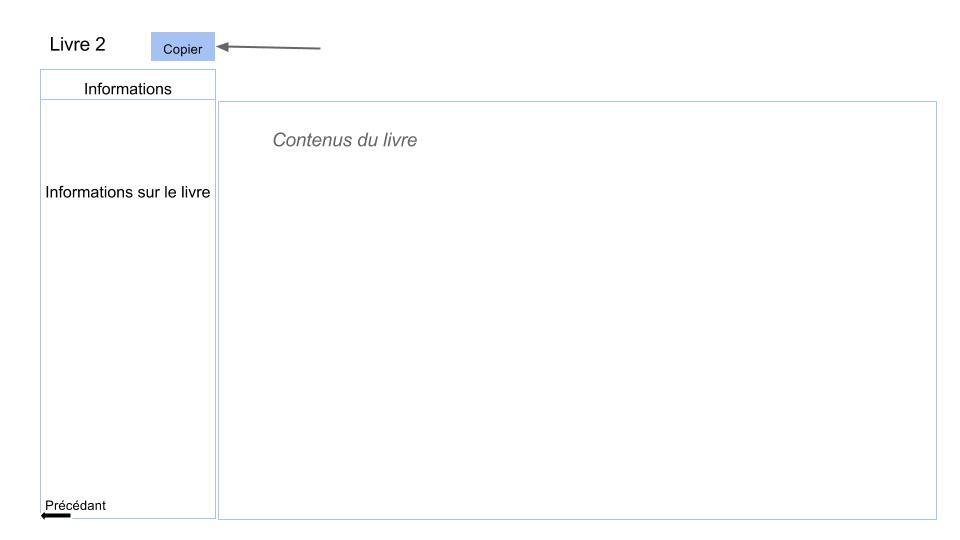
\includegraphics[width=\textwidth]{creer_livre}
\caption{Créer un projet à partir d'un livre}
\end{figure}

\begin{figure}[H]
\centering
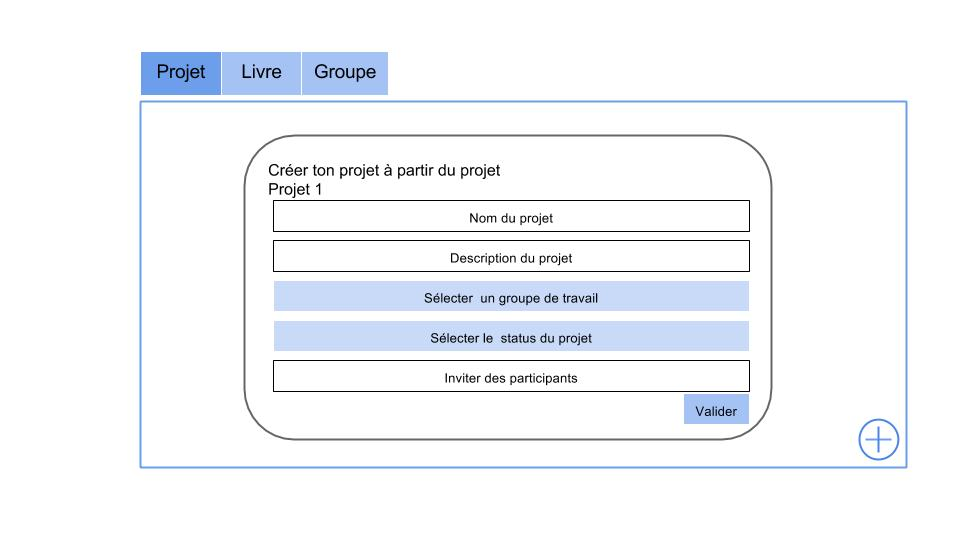
\includegraphics[width=\textwidth]{creer_info}
\caption{Remplir toutes les informations demandées}
\end{figure}

\subsection{Distribuer un projet}

Sur la page d'un layer original, à droite il y a toutes les séquences ; quand on crée des séquences on sélectionne des éditeurs, mais on peut aussi sélectionner des éditeurs pour d'autres séquences quand on entre dans l'édition de la séquence ; il suffit de cliquer sur l'icône plus.

\begin{figure}[H]
\centering
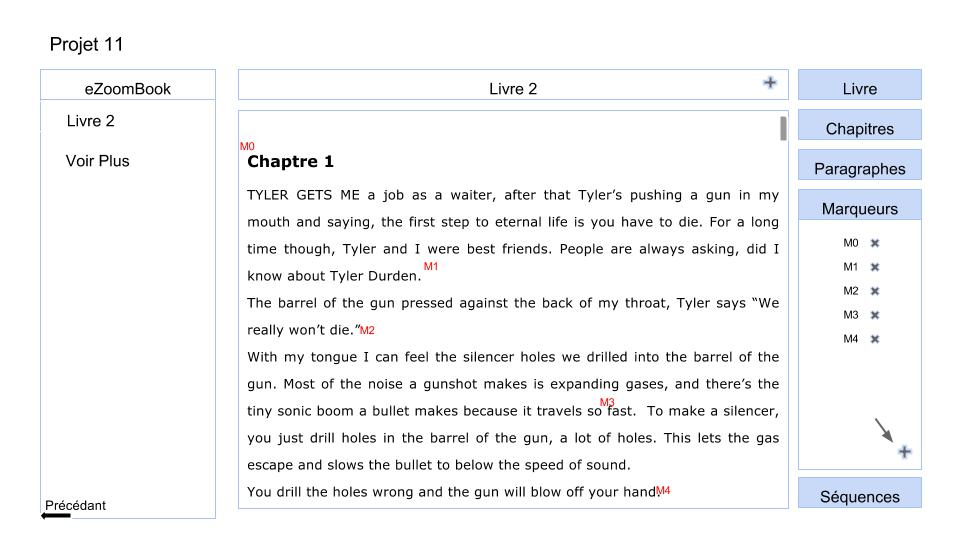
\includegraphics[width=\textwidth]{marqueurs}
\caption{Créer des marqueurs}
\end{figure}

\begin{figure}[H]
\centering
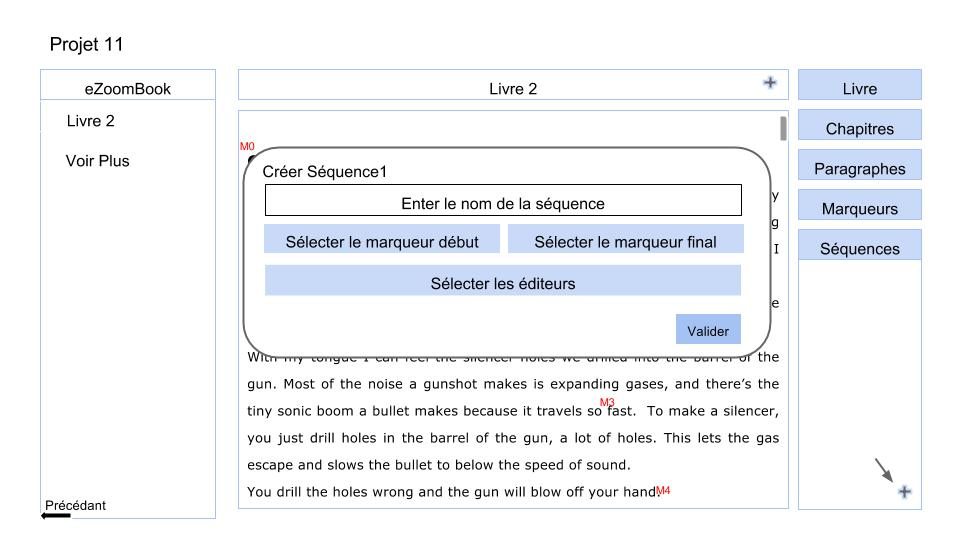
\includegraphics[width=\textwidth]{sequences}
\caption{Créer des séquences}
\end{figure}

\begin{figure}[H]
\centering
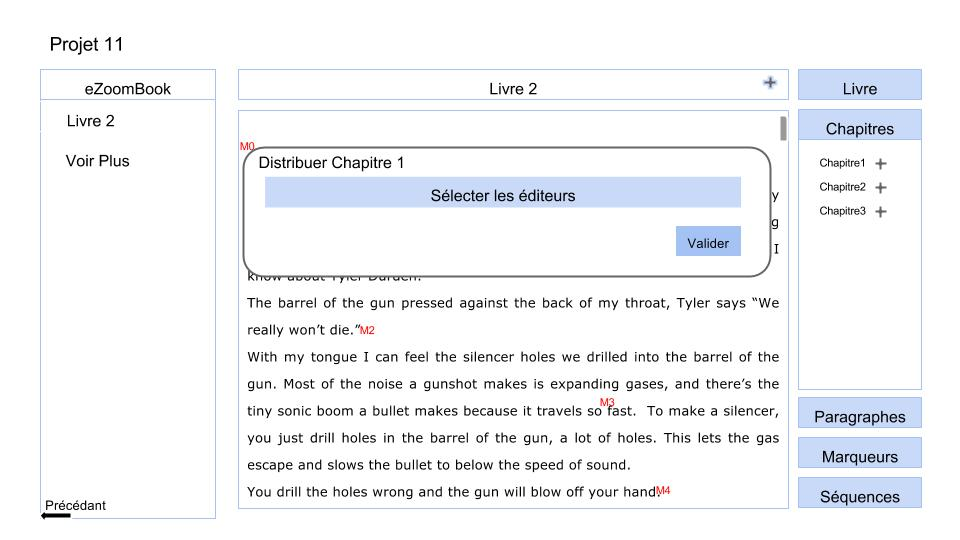
\includegraphics[width=\textwidth]{distribuer}
\caption{Distribuer des chapitres}
\end{figure}

\subsection{Contribuer dans un projet}

\subsubsection{Créer un layer}

Quand on créé un sous-layer à partir d'un layer original, il faut choisir les séquences, mais si on créé un sous-layer à partir d'un layer travail, celui-ci hérite automatiquement de la ségmentation de son parent layer.

\begin{figure}[H]
\centering
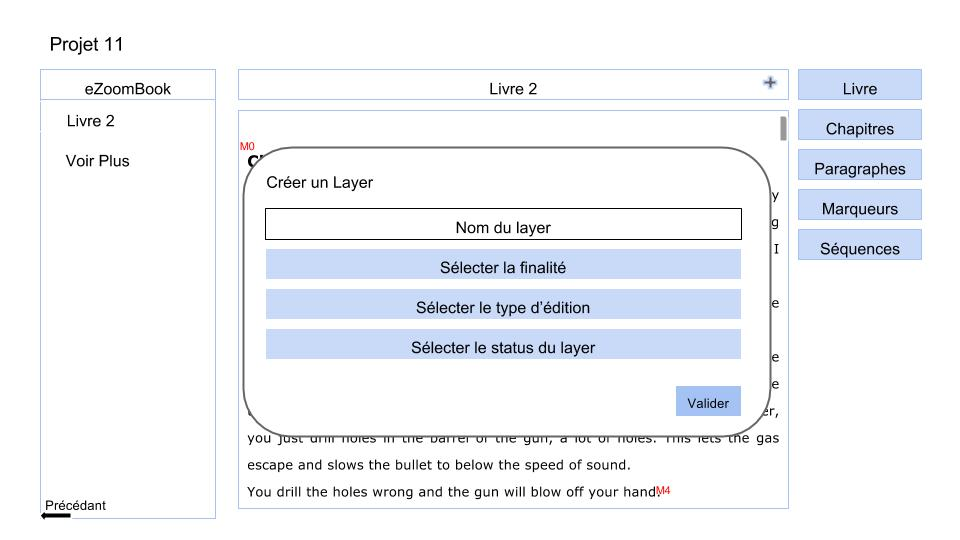
\includegraphics[width=\textwidth]{creer_layer}
\caption{Informations à remplir pour la création d'un sous-layer à partir d'un layer original}
\end{figure}

\begin{figure}[H]
\centering
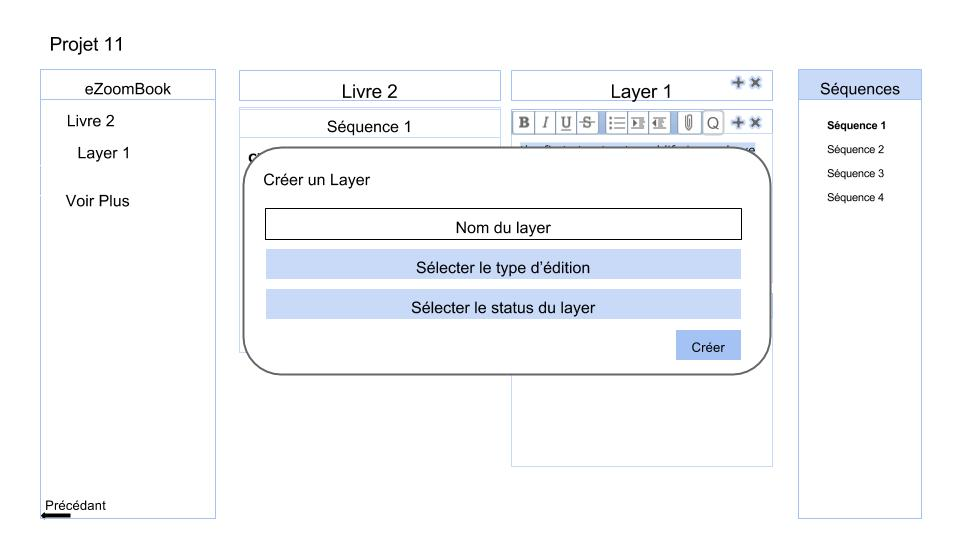
\includegraphics[width=\textwidth]{creer_commentaire}
\caption{Informations à remplir d'une création d'un sous-layer d'un layer travail}
\end{figure}

\subsubsection{Editer un layer}

Après le processus de création, on va rentrer directement dans le processus de contribution du layer. Sur la page de contribution, le layer est mis à doite et son parent layer est à gauche ce qui permet un travail sur ces documents assez simple. Dans l'édition d'un layer, on peut aussi sélectionner tous les layers de niveau supérieur en sélecttionnant le nom du layer à gauche.

Dans les blocks permettant plusieurs types de manipulations, on peut faire des citations, écrire en multiformat et insérer des images, etc. C'est aussi possible d'insérer des parties en cliquant sur les petites icônes plus ; et la nouvelle partie viendra s'insérer entre celle sur laquelle on travaille et la partie précédente. Il est possible d'utiliser l'icône croix lorsqu'on veut éditer uniquement certaines parties d'un livre : pour ne garder que les séquences souhaitées, il suffit de cliquer sur la petite croix qui permet de supprimer une séquence. Si on veut faire une citation, il suffit de cliquer sur le boutton Q et sélectionner une partie à partir du parent layer.

\begin{figure}[H]
\centering
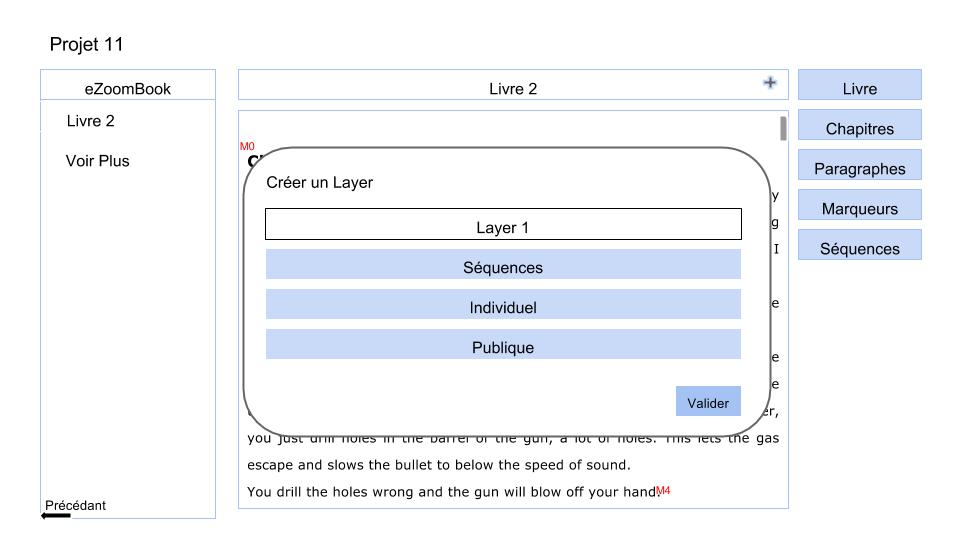
\includegraphics[width=\textwidth]{creer_indi}
\caption{Créer un layer individuel}
\end{figure}

\begin{figure}[H]
\centering
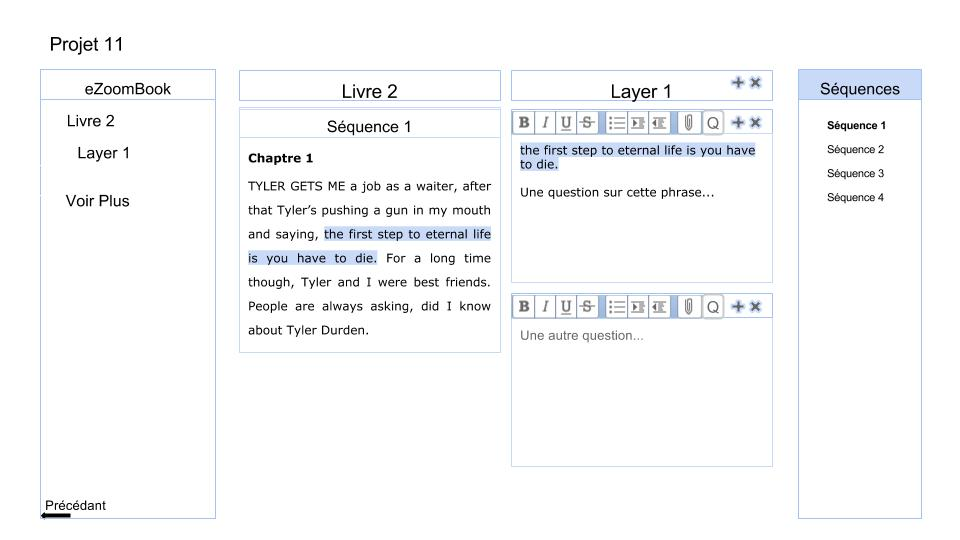
\includegraphics[width=\textwidth]{edition_indi}
\caption{Editer le layer individuel}
\end{figure}

\begin{figure}[H]
\centering
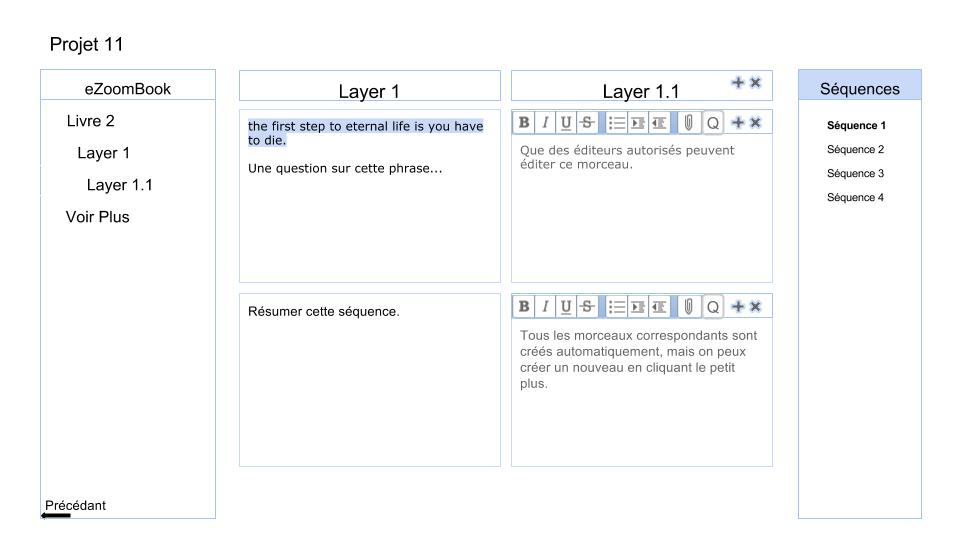
\includegraphics[width=\textwidth]{col_parent}
\caption{Un layer avec son parent layer}
\end{figure}

\begin{figure}[H]
\centering
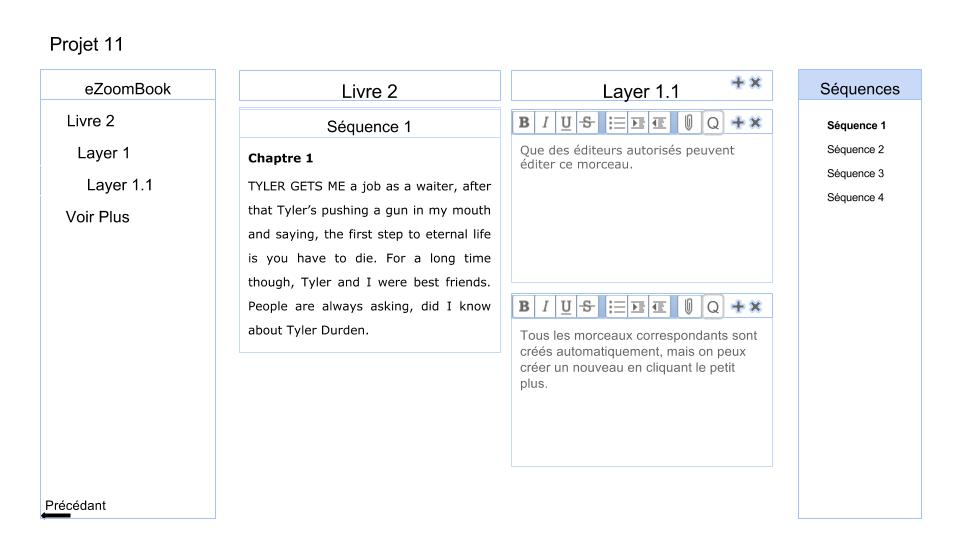
\includegraphics[width=\textwidth]{col}
\caption{Le layer avec son layer original}
\end{figure}